% Lines and a cap in F_3^2 (generated by figs_c1ch11.py).
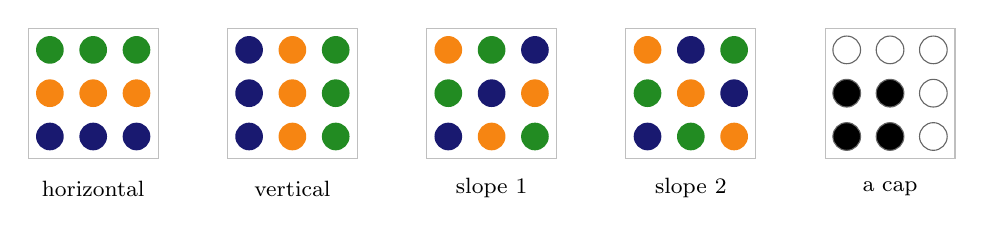
\begin{tikzpicture}[x=0.55cm,y=0.55cm,l/.style={font=\footnotesize}]
\draw[black!25] (-0.5,-0.5) rectangle (2.5,2.5);
\fill[MidnightBlue] (0.0,0) circle (5pt);
\fill[BurntOrange] (0.0,1) circle (5pt);
\fill[ForestGreen] (0.0,2) circle (5pt);
\fill[MidnightBlue] (1.0,0) circle (5pt);
\fill[BurntOrange] (1.0,1) circle (5pt);
\fill[ForestGreen] (1.0,2) circle (5pt);
\fill[MidnightBlue] (2.0,0) circle (5pt);
\fill[BurntOrange] (2.0,1) circle (5pt);
\fill[ForestGreen] (2.0,2) circle (5pt);
\node[l] at (1.0,-1.2) {horizontal};
\draw[black!25] (4.1,-0.5) rectangle (7.1,2.5);
\fill[MidnightBlue] (4.6,0) circle (5pt);
\fill[MidnightBlue] (4.6,1) circle (5pt);
\fill[MidnightBlue] (4.6,2) circle (5pt);
\fill[BurntOrange] (5.6,0) circle (5pt);
\fill[BurntOrange] (5.6,1) circle (5pt);
\fill[BurntOrange] (5.6,2) circle (5pt);
\fill[ForestGreen] (6.6,0) circle (5pt);
\fill[ForestGreen] (6.6,1) circle (5pt);
\fill[ForestGreen] (6.6,2) circle (5pt);
\node[l] at (5.6,-1.2) {vertical};
\draw[black!25] (8.7,-0.5) rectangle (11.7,2.5);
\fill[MidnightBlue] (9.2,0) circle (5pt);
\fill[ForestGreen] (9.2,1) circle (5pt);
\fill[BurntOrange] (9.2,2) circle (5pt);
\fill[BurntOrange] (10.2,0) circle (5pt);
\fill[MidnightBlue] (10.2,1) circle (5pt);
\fill[ForestGreen] (10.2,2) circle (5pt);
\fill[ForestGreen] (11.2,0) circle (5pt);
\fill[BurntOrange] (11.2,1) circle (5pt);
\fill[MidnightBlue] (11.2,2) circle (5pt);
\node[l] at (10.2,-1.2) {slope $1$};
\draw[black!25] (13.299999999999999,-0.5) rectangle (16.299999999999997,2.5);
\fill[MidnightBlue] (13.799999999999999,0) circle (5pt);
\fill[ForestGreen] (13.799999999999999,1) circle (5pt);
\fill[BurntOrange] (13.799999999999999,2) circle (5pt);
\fill[ForestGreen] (14.799999999999999,0) circle (5pt);
\fill[BurntOrange] (14.799999999999999,1) circle (5pt);
\fill[MidnightBlue] (14.799999999999999,2) circle (5pt);
\fill[BurntOrange] (15.799999999999999,0) circle (5pt);
\fill[MidnightBlue] (15.799999999999999,1) circle (5pt);
\fill[ForestGreen] (15.799999999999999,2) circle (5pt);
\node[l] at (14.799999999999999,-1.2) {slope $2$};
\draw[black!25] (17.9,-0.5) rectangle (20.9,2.5);
\filldraw[draw=black!60,fill=black] (18.4,0) circle (5pt);
\filldraw[draw=black!60,fill=black] (18.4,1) circle (5pt);
\filldraw[draw=black!60,fill=white] (18.4,2) circle (5pt);
\filldraw[draw=black!60,fill=black] (19.4,0) circle (5pt);
\filldraw[draw=black!60,fill=black] (19.4,1) circle (5pt);
\filldraw[draw=black!60,fill=white] (19.4,2) circle (5pt);
\filldraw[draw=black!60,fill=white] (20.4,0) circle (5pt);
\filldraw[draw=black!60,fill=white] (20.4,1) circle (5pt);
\filldraw[draw=black!60,fill=white] (20.4,2) circle (5pt);
\node[l] at (19.4,-1.2) {a cap};
\end{tikzpicture}
